% Options for packages loaded elsewhere
\PassOptionsToPackage{unicode}{hyperref}
\PassOptionsToPackage{hyphens}{url}
%
\documentclass[
]{book}
\usepackage{amsmath,amssymb}
\usepackage{lmodern}
\usepackage{iftex}
\ifPDFTeX
  \usepackage[T1]{fontenc}
  \usepackage[utf8]{inputenc}
  \usepackage{textcomp} % provide euro and other symbols
\else % if luatex or xetex
  \usepackage{unicode-math}
  \defaultfontfeatures{Scale=MatchLowercase}
  \defaultfontfeatures[\rmfamily]{Ligatures=TeX,Scale=1}
\fi
% Use upquote if available, for straight quotes in verbatim environments
\IfFileExists{upquote.sty}{\usepackage{upquote}}{}
\IfFileExists{microtype.sty}{% use microtype if available
  \usepackage[]{microtype}
  \UseMicrotypeSet[protrusion]{basicmath} % disable protrusion for tt fonts
}{}
\makeatletter
\@ifundefined{KOMAClassName}{% if non-KOMA class
  \IfFileExists{parskip.sty}{%
    \usepackage{parskip}
  }{% else
    \setlength{\parindent}{0pt}
    \setlength{\parskip}{6pt plus 2pt minus 1pt}}
}{% if KOMA class
  \KOMAoptions{parskip=half}}
\makeatother
\usepackage{xcolor}
\usepackage{color}
\usepackage{fancyvrb}
\newcommand{\VerbBar}{|}
\newcommand{\VERB}{\Verb[commandchars=\\\{\}]}
\DefineVerbatimEnvironment{Highlighting}{Verbatim}{commandchars=\\\{\}}
% Add ',fontsize=\small' for more characters per line
\usepackage{framed}
\definecolor{shadecolor}{RGB}{248,248,248}
\newenvironment{Shaded}{\begin{snugshade}}{\end{snugshade}}
\newcommand{\AlertTok}[1]{\textcolor[rgb]{0.94,0.16,0.16}{#1}}
\newcommand{\AnnotationTok}[1]{\textcolor[rgb]{0.56,0.35,0.01}{\textbf{\textit{#1}}}}
\newcommand{\AttributeTok}[1]{\textcolor[rgb]{0.77,0.63,0.00}{#1}}
\newcommand{\BaseNTok}[1]{\textcolor[rgb]{0.00,0.00,0.81}{#1}}
\newcommand{\BuiltInTok}[1]{#1}
\newcommand{\CharTok}[1]{\textcolor[rgb]{0.31,0.60,0.02}{#1}}
\newcommand{\CommentTok}[1]{\textcolor[rgb]{0.56,0.35,0.01}{\textit{#1}}}
\newcommand{\CommentVarTok}[1]{\textcolor[rgb]{0.56,0.35,0.01}{\textbf{\textit{#1}}}}
\newcommand{\ConstantTok}[1]{\textcolor[rgb]{0.00,0.00,0.00}{#1}}
\newcommand{\ControlFlowTok}[1]{\textcolor[rgb]{0.13,0.29,0.53}{\textbf{#1}}}
\newcommand{\DataTypeTok}[1]{\textcolor[rgb]{0.13,0.29,0.53}{#1}}
\newcommand{\DecValTok}[1]{\textcolor[rgb]{0.00,0.00,0.81}{#1}}
\newcommand{\DocumentationTok}[1]{\textcolor[rgb]{0.56,0.35,0.01}{\textbf{\textit{#1}}}}
\newcommand{\ErrorTok}[1]{\textcolor[rgb]{0.64,0.00,0.00}{\textbf{#1}}}
\newcommand{\ExtensionTok}[1]{#1}
\newcommand{\FloatTok}[1]{\textcolor[rgb]{0.00,0.00,0.81}{#1}}
\newcommand{\FunctionTok}[1]{\textcolor[rgb]{0.00,0.00,0.00}{#1}}
\newcommand{\ImportTok}[1]{#1}
\newcommand{\InformationTok}[1]{\textcolor[rgb]{0.56,0.35,0.01}{\textbf{\textit{#1}}}}
\newcommand{\KeywordTok}[1]{\textcolor[rgb]{0.13,0.29,0.53}{\textbf{#1}}}
\newcommand{\NormalTok}[1]{#1}
\newcommand{\OperatorTok}[1]{\textcolor[rgb]{0.81,0.36,0.00}{\textbf{#1}}}
\newcommand{\OtherTok}[1]{\textcolor[rgb]{0.56,0.35,0.01}{#1}}
\newcommand{\PreprocessorTok}[1]{\textcolor[rgb]{0.56,0.35,0.01}{\textit{#1}}}
\newcommand{\RegionMarkerTok}[1]{#1}
\newcommand{\SpecialCharTok}[1]{\textcolor[rgb]{0.00,0.00,0.00}{#1}}
\newcommand{\SpecialStringTok}[1]{\textcolor[rgb]{0.31,0.60,0.02}{#1}}
\newcommand{\StringTok}[1]{\textcolor[rgb]{0.31,0.60,0.02}{#1}}
\newcommand{\VariableTok}[1]{\textcolor[rgb]{0.00,0.00,0.00}{#1}}
\newcommand{\VerbatimStringTok}[1]{\textcolor[rgb]{0.31,0.60,0.02}{#1}}
\newcommand{\WarningTok}[1]{\textcolor[rgb]{0.56,0.35,0.01}{\textbf{\textit{#1}}}}
\usepackage{longtable,booktabs,array}
\usepackage{calc} % for calculating minipage widths
% Correct order of tables after \paragraph or \subparagraph
\usepackage{etoolbox}
\makeatletter
\patchcmd\longtable{\par}{\if@noskipsec\mbox{}\fi\par}{}{}
\makeatother
% Allow footnotes in longtable head/foot
\IfFileExists{footnotehyper.sty}{\usepackage{footnotehyper}}{\usepackage{footnote}}
\makesavenoteenv{longtable}
\usepackage{graphicx}
\makeatletter
\def\maxwidth{\ifdim\Gin@nat@width>\linewidth\linewidth\else\Gin@nat@width\fi}
\def\maxheight{\ifdim\Gin@nat@height>\textheight\textheight\else\Gin@nat@height\fi}
\makeatother
% Scale images if necessary, so that they will not overflow the page
% margins by default, and it is still possible to overwrite the defaults
% using explicit options in \includegraphics[width, height, ...]{}
\setkeys{Gin}{width=\maxwidth,height=\maxheight,keepaspectratio}
% Set default figure placement to htbp
\makeatletter
\def\fps@figure{htbp}
\makeatother
\setlength{\emergencystretch}{3em} % prevent overfull lines
\providecommand{\tightlist}{%
  \setlength{\itemsep}{0pt}\setlength{\parskip}{0pt}}
\setcounter{secnumdepth}{5}
\usepackage{booktabs}
\ifLuaTeX
  \usepackage{selnolig}  % disable illegal ligatures
\fi
\usepackage[]{natbib}
\bibliographystyle{apalike}
\IfFileExists{bookmark.sty}{\usepackage{bookmark}}{\usepackage{hyperref}}
\IfFileExists{xurl.sty}{\usepackage{xurl}}{} % add URL line breaks if available
\urlstyle{same} % disable monospaced font for URLs
\hypersetup{
  pdftitle={BIOL 3295: Population and Evolutionary Ecology, Winter 2023},
  pdfauthor={Amy Hurford},
  hidelinks,
  pdfcreator={LaTeX via pandoc}}

\title{BIOL 3295: Population and Evolutionary Ecology, Winter 2023}
\author{Amy Hurford}
\date{2023-01-13}

\begin{document}
\maketitle

{
\setcounter{tocdepth}{1}
\tableofcontents
}
\hypertarget{syllabus}{%
\chapter{Syllabus}\label{syllabus}}

\hypertarget{instructor-information}{%
\section{Instructor Information}\label{instructor-information}}

Instructor: Dr.~Amy Hurford\\
Office: CSF 4338\\
Email: \href{mailto:ahurford@mun.ca}{\nolinkurl{ahurford@mun.ca}}\\
I will try to reply to emails within 24 hours (excluding evenings, weekends and holidays).
Office hours: Tuesday 1-2pm; Thursday 1-2pm

\hypertarget{course-information}{%
\section{Course Information}\label{course-information}}

TR 12.00-12.50pm\\
F 1-1.50pm\\
Classroom: SN3060~(unless stated otherwise on the schedule)

All Course Announcements will be made on BrightSpace. Should lectures be remote a WebEx link will be provided on BrightSpace.

Course description:\\
Population and Evolutionary Ecology is an introduction to the theory and principles of evolutionary ecology and population dynamics. Pre-requisites: BIOL 2600; at least one of BIOL 2010, 2122 or 2210.\\

Course format:\\
The course consists of lectures, 4 data analysis assignments, 2 exams and a final exam.~

Course expectations:\\
Please attend lectures and respect the learning environment of other students. If you have COVID-19 please follow university and provincial public health guidelines.\\

Learning goals:\\
The course content emphasizes a deeper understanding of fewer concepts. You have seen much of the course material in pre-requisite courses. In this course, I will revisit the models, clarify the assumptions and when they are appropriate, and we will fit the models to data to estimate parameters. By the end of the course, I hope that if you were given population data, that you would know the key quantities that you might estimate, and could complete the analysis.

Required Text and Resources:\\
The course materials are online at \url{https://ahurford.github.io/biol-3295-winter-2023/index.html}.

Most readings are assigned from two textbooks that are available electronically from the library:

\begin{itemize}
\item
  Vandermeer, J.H., Goldberg, D.E., 2013. Population Ecology: First Principles (Second Edition). Princeton University Press, Princeton, United States. \href{https://ebookcentral-proquest-com.qe2a-proxy.mun.ca/lib/mun/detail.action?docID=1205619}{Link}
\item
  Otto, Sarah P., and Troy Day. 2007. A Biologist's Guide to Mathematical Modeling in Ecology and Evolution, Princeton University Press. \href{https://ebookcentral-proquest-com.qe2a-proxy.mun.ca/lib/mun/detail.action?docID=768551}{Link}
\end{itemize}

If you wish to use your own computer for assignments you should install \texttt{R} and \texttt{RStudio} (see also \href{https://ahurford.github.io/quant-guide-all-courses/install.html}{here}).

\hypertarget{method-of-evaluation}{%
\section{Method of Evaluation}\label{method-of-evaluation}}

\begin{itemize}
\tightlist
\item
  4 Assignments - 20\%\\
\item
  2 Exams - 40\%\\
\item
  Final Exam - 40\%\\
\end{itemize}

Late assignments and missed exams, and final exams will be accommodated as described by University Regulation 6.7.3 and 6.7.5 (see \url{https://www.mun.ca/regoff/calendar/sectionNo=REGS-0474} for Regulations). Please discuss missed assignments and exams with me. To accommodate the absence an assignment may be modified or exempted and re-weighted in the grading scheme.

\hypertarget{additional-policies}{%
\section{Additional Policies}\label{additional-policies}}

\hypertarget{accommodation-of-students-with-disabilities}{%
\subsection{Accommodation of students with disabilities}\label{accommodation-of-students-with-disabilities}}

Memorial University of Newfoundland is committed to supporting inclusive education based on the principles of equity, accessibility and collaboration. Accommodations are provided within the scope of the University Policies for the Accommodations for Students with Disabilities see \url{www.mun.ca/policy/site/policy.php?id=239}. Students who may need an academic accommodation are asked to initiate the request with the Glenn Roy Blundon Centre at the earliest opportunity (see \url{www.mun.ca/blundon} for more information).

\hypertarget{academic-misconduct}{%
\subsection{Academic misconduct}\label{academic-misconduct}}

Students are expected to adhere to those principles, which constitute proper academic conduct. A student has the responsibility to know which actions, as described under Academic Offences in the University Regulations, could be construed as dishonest or improper. Students found guilty of an academic offence may be subject to a number of penalties commensurate with the offence including reprimand, reduction of grade, probation, suspension or expulsion from the University. For more information regarding this policy, students should refer to University Regulation 6.12.

\hypertarget{equity-and-diversity}{%
\subsection{Equity and Diversity}\label{equity-and-diversity}}

A safe learning environment will be provided for all students regardless of race, colour, nationality, ethnic origin, social origin, religious creed, religion, age, disability, disfigurement, sex (including pregnancy), sexual orientation, gender identity, gender expression, marital status, family status, source of income or political opinion.

You should not photograph or record myself, teaching assistants, or other students in the class without first obtaining permission. Accommodation will be made for students with special needs.

The sound should be turned off on phones and computers during class.

\hypertarget{additional-supports}{%
\section{Additional Supports}\label{additional-supports}}

Resources for additional support can be found at:

\begin{itemize}
\item
  \url{www.mun.ca/currentstudents/student/}
\item
  \url{https://munsu.ca/resource-centres/}
\end{itemize}

\hypertarget{schedule}{%
\chapter{Schedule}\label{schedule}}

All lectures are in SN 3060 unless otherwise stated

\begin{itemize}
\tightlist
\item
  Thurs Jan 5: Introduction
\item
  Fri Jan 6: Population biology with discrete and continuous variables
\item
  Tues Jan 10: ---
\item
  Thurs Jan 12: \textbf{CSF 2218} Introduction to Rmarkdown and tidyverse \textbf{Assignment 1 is assigned}
\item
  Fri Jan 13: Geometric growth
\item
  Tues Jan 17: Exponential growth
\item
  Thurs Jan 19: \textbf{CSF 2218} Numerical solutions and graphing population data \textbf{Assignment 2 is assigned}
\item
  Fri Jan 20: Exponential growth
\item
  Tues Jan 24: Density dependence and logistic growth
\item
  Thurs Jan 26: Density dependence and logistic growth \textbf{Assignments 1 \& 2 are due}
\item
  Fri Jan 27: Density dependence and logistic growth
\item
  Tues Jan 31: Discrete time density dependence
\item
  Thurs Feb 2: \textbf{EXAM I} (all material covered to date)
\item
  Fri Feb 3: Age-structured models
\item
  Tues Feb 7: Stage-structured models
\item
  Thurs Feb 9: Stage-structured models
\item
  Fri Feb 10: Stage-structured models
\item
  Tues Feb 14: \textbf{CSF 2218} Numerical analysis of stage-structured models \textbf{Assignment 3 is assigned}
\item
  Thurs Feb 16: Density dependence in stage-structured models
\item
  Fri Feb 17: Metapopulation models
\end{itemize}

WINTER BREAK

\begin{itemize}
\tightlist
\item
  Tues Feb 28: Continuous space models \textbf{Assignment 3 is due}
\item
  Thurs Mar 2: Spatially explicit models in population biology
\item
  Fri Mar 3: Population dynamics in a warming world
\item
  Tues Mar 7: Spatially explicit population dynamics in a warming world
\item
  Thurs Mar 9: Disease dynamics
\item
  Fri Mar 10: The net reproduction number
\item
  Tues Mar 14: Overview of models in population biology
\item
  Thurs Mar 16: \textbf{EXAM II} (All material since Exam I)
\item
  Fri Mar 17: What is evolutionary ecology?
\item
  Tues Mar 21: Haploid selection model
\item
  Thur Mar 23: \href{https://www.zoology.ubc.ca/~otto/Talks/SSE2022_Otto.pdf}{Selection coefficients for COVID-19 variants}
\item
  Fri Mar 24: \textbf{CSF 2218} Estimating selection coefficients \textbf{Assignment 4 is assigned}
\item
  Tues Mar 28: The evolutionary ecology of pathogens
\item
  Thurs Mar 30: The evolutionary ecology of COVID-19
\item
  Fri Mar 31: The evolutionary ecology of hosts \textbf{Assignment 4 is due}
\item
  Tues Apr 3: The evolution of reproductive effort in plants
\item
  Thurs Apr 5: Evolutionarily stable and convergent stable strategies
\item
  Fri Apr 6: Review
\end{itemize}

TBD \textbf{FINAL EXAM} (all course material)

\hypertarget{jan-5-introduction}{%
\chapter{Jan 5: Introduction}\label{jan-5-introduction}}

\begin{itemize}
\tightlist
\item
  Survey of student computer preferences
\end{itemize}

\hypertarget{some-questions}{%
\section{Some questions}\label{some-questions}}

\begin{itemize}
\tightlist
\item
  What is a population?
\item
  What are some definitions of a population that are given in textbooks?
\item
  In research studies, how are populations discussed in the \emph{Discussion}?
\item
  How are individuals that comprise the sample selected in the \emph{Methods} of a research study?
\item
  List some potential differences between how populations are defined and discussed and the research methods?
\item
  Why does the definition of a population matter?
\end{itemize}

\hypertarget{references}{%
\section{References}\label{references}}

Vandermeer, J.H., Goldberg, D.E., 2013. Population Ecology: First Principles (Second Edition). Princeton University Press, Princeton, United States. \href{https://ebookcentral-proquest-com.qe2a-proxy.mun.ca/lib/mun/detail.action?docID=1205619}{Link}

The Princeton Guide to Ecology, edited by Simon A. Levin, et al., Princeton University Press, 2009. ProQuest Ebook Central, \href{https://ebookcentral-proquest-com.qe2a-proxy.mun.ca/lib/mun/detail.action?docID=557123}{Link}

Sacchi, R., Gentilli, A., Razzetti, E., Barbieri, F., 2002. Effects of building features on density and flock distribution of feral pigeons Columba livia var. domestica in an urban environment. Can. J. Zool. 80, 48-54. \href{https://cdnsciencepub.com/doi/10.1139/z01-202}{Link}

\hypertarget{jan-6-discrete-and-continous-variables}{%
\chapter{Jan 6: Discrete and continous variables}\label{jan-6-discrete-and-continous-variables}}

Reading: Otto, Sarah P., and Troy Day. 2007. A Biologist's Guide to Mathematical Modeling in Ecology and Evolution, Princeton University Press. \href{https://ebookcentral-proquest-com.qe2a-proxy.mun.ca/lib/mun/detail.action?docID=768551}{Link} \textbf{pages 33-38 in Section 2.3}

\begin{itemize}
\item
  Parameters versus variables
\item
  Fitted versus independently estimated parameters
\end{itemize}

\hypertarget{jan-12-assignment-rmarkdown-and-tidyverse}{%
\chapter{\texorpdfstring{Jan 12: \textbf{ASSIGNMENT} Rmarkdown and tidyverse}{Jan 12: ASSIGNMENT Rmarkdown and tidyverse}}\label{jan-12-assignment-rmarkdown-and-tidyverse}}

(Dates changed owing to the university closure for a snow day)

ASSIGNMENT 1 due Jan 26.

\textbf{PART I} is to reproduce a figure and the figure caption of a plot in \href{https://ebookcentral-proquest-com.qe2a-proxy.mun.ca/lib/mun/detail.action?docID=1205619}{Vandermeer and Goldberg 2013} or another textbook or a published paper in Rmarkdown and as an output file: .hmtl, .pdf, or .docx. Please choose a figure to reproduce in the area of Population Biology or Evolutionary Ecology.

You can simplify a complex figure if necessary. Your figure should be made in \texttt{ggplot()} and have:

\begin{itemize}
\item
  the title (if there is one),
\item
  axes labels,
\item
  points or lines or both,
\item
  approximately the same data as the original figure,
\item
  the correct axes limits.
\end{itemize}

The objective is for you to learn how to use Rmarkdown to make a synthetic write-up that includes code, a figure and text. Your completed output should have:

\begin{enumerate}
\def\labelenumi{\arabic{enumi}.}
\tightlist
\item
  A brief text description of where I can find the figure you reproduced.
\item
  Code that makes a figure that is suppressed in the output file.
\item
  The reproduced figure (or simplified figure).
\item
  The actual figure
\end{enumerate}

You are to hand-in the \texttt{.Rmd} file and an output file (\texttt{.html}, \texttt{.pdf}, or \texttt{.docx})

Here, is an example of what a completed PART 1 looks like (as an .html output).

\begin{center}\rule{0.5\linewidth}{0.5pt}\end{center}

The graph is Figure 3.1 from \href{https://ebookcentral-proquest-com.qe2a-proxy.mun.ca/lib/mun/detail.action?docID=1205619}{Population Ecology: First Principles - Second Edition (Vandermeer and Goldberg)} on p67.

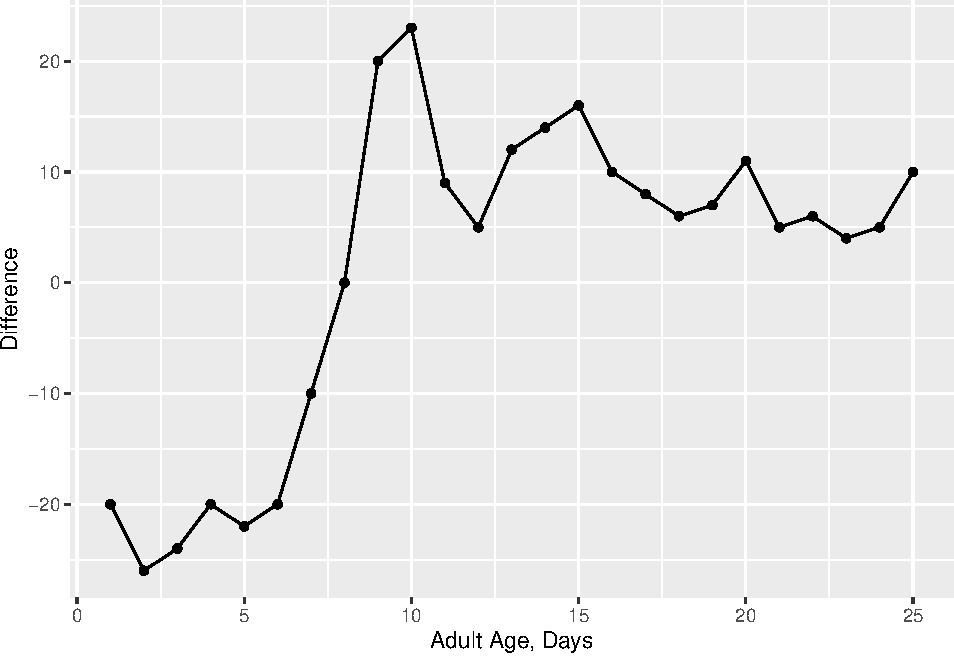
\includegraphics{BIOL-3295_files/figure-latex/unnamed-chunk-1-1.pdf}

\textbf{FIGURE 3.1} Difference in per capita egg production between the O lines and B lines from Rose and Charlesworth's (1981) experiment.

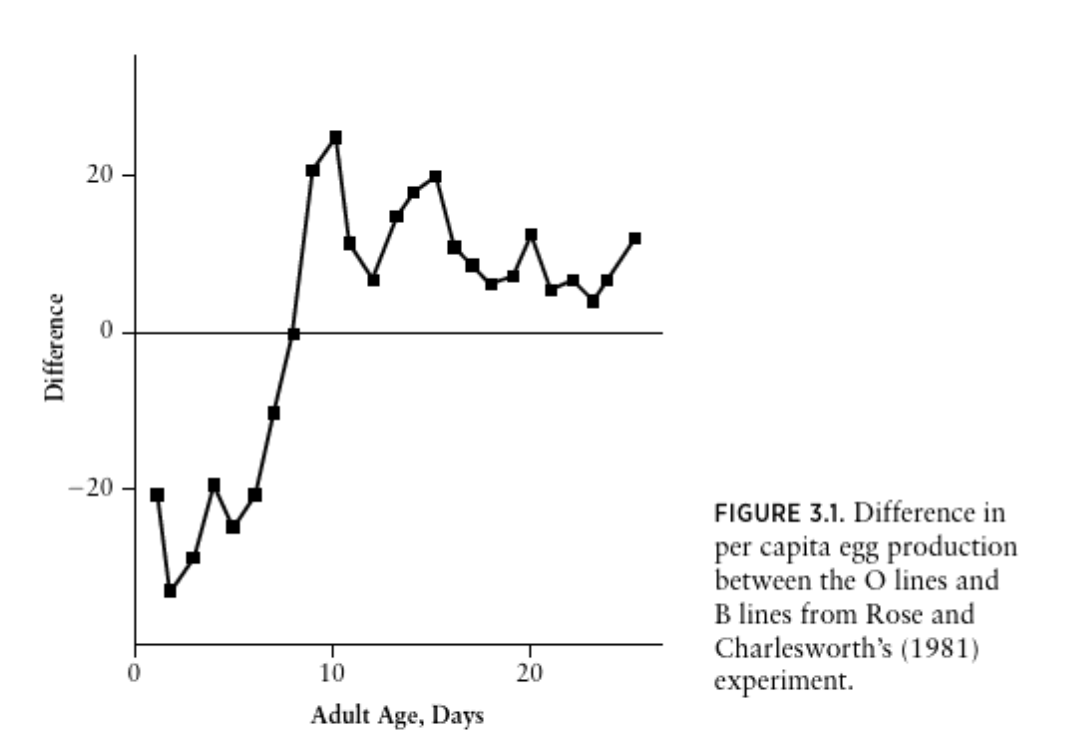
\includegraphics[width=0.9\linewidth]{figures/actual-fig}

\begin{center}\rule{0.5\linewidth}{0.5pt}\end{center}

Instructions to complete PART I are \protect\hyperlink{partI}{here}.

\textbf{PART II} of this assignment is to clean up messy data. As a biologist, much of my coding work involves getting data into the right format to use in functions, this might be a plot function like \texttt{ggplot()}, which you used in PART I, or a statistical function like \texttt{lm()}, which will perform a regression, t-test, or analysis of variance. The objective of PART II is to practice cleaning messy data into a useable format.

\begin{enumerate}
\def\labelenumi{\arabic{enumi}.}
\tightlist
\item
  You are to clean the messy data from \href{https://datacarpentry.org/semester-biology/exercises/Tidy-data-improving-messy-data-SQL/}{here} enough so you can make a plot using \texttt{ggplot()}. Some helpful instructions for how to do this are \protect\hyperlink{partII}{here}. The code that you write \textbf{must use the \texttt{select()}, \texttt{mutate()}, and \texttt{ggplot()} functions}. The graph that you make must be different than the example given in the instructions - for example, you might plot the same variables but for Plot 2.
\end{enumerate}

(perhaps this sounds easy - this data is pretty messy - I found it quite hard!)

\textbf{TO HAND IN}

\begin{enumerate}
\def\labelenumi{\arabic{enumi}.}
\tightlist
\item
  Hand in an \texttt{.Rmd} file and an output file (\texttt{.html}, \texttt{.docx}, or \texttt{.pdf}) with the solutions to both PART I and PART II of this assignment. Each part is 10 marks for a total of 20 marks.
\end{enumerate}

\hypertarget{jan-13-geometric-growth}{%
\chapter{Jan 13: Geometric growth}\label{jan-13-geometric-growth}}

\hypertarget{reading}{%
\section{Reading}\label{reading}}

Vandermeer, J.H., Goldberg, D.E., 2013. Population Ecology: First Principles (Second Edition). Princeton University Press, Princeton, United States. \textbf{p1-3.} \href{https://ebookcentral-proquest-com.qe2a-proxy.mun.ca/lib/mun/detail.action?docID=1205619}{Link}

\begin{itemize}
\item
  Von Foerster human population become effectively infinite on Nov 13 2026
\item
  Lilly pads replicate once per week. If it take a year for 1/2 a pond to be covered, when will it be completely covered? See also the \href{https://en.wikipedia.org/wiki/Wheat_and_chessboard_problem}{wheat and chessboard}
\item
  \(N_{t+1} = \lambda N_t\) equation 3 in \href{https://ebookcentral-proquest-com.qe2a-proxy.mun.ca/lib/mun/detail.action?docID=1205619}{Vandermeer and Goldberg}. For what values of \(\lambda\) will the population size, \(N_t\), grow?
\item
  \(N_t = N_0 \lambda^t\) is equation 4 in \href{https://ebookcentral-proquest-com.qe2a-proxy.mun.ca/lib/mun/detail.action?docID=1205619}{Vandermeer and Goldberg} (but written more generally). With \(N_0 > 0\) sketch a graph of \(N_t\) for different values of \(\lambda\). If \(N_0 = 0\), sketch a graph of \(N_t\).
\item
  If \(N_0 = 1.1\) individuals per km\(^2\), \(\lambda = 2\), what is is the population size at time \(t = 10\)?
\item
  Consider population growth of pheasants on \protect\hyperlink{pheasant}{Protection Island}. If we were to apply the geometric growth model to the pheasant population, what are some assumptions? How might this affect our parameterization (i.e., our estimate of \(\lambda\)) for the pheasant population?
\item
  How can we understand what \(\lambda\) is in a population that has births and deaths?
\end{itemize}

\hypertarget{pheasant}{%
\chapter{Jan 17: Geometric growth}\label{pheasant}}

\hypertarget{reading-1}{%
\section{Reading}\label{reading-1}}

Download the .pdf of the MSc thesis below and read the Abstract (the first two pages prior to the title page). Pay specific attention to the number of pheasants at different points in time, these might be \(N_{t+1}\) and \(N_t\) in the geometric growth model formula; and the number of births and deaths that occur, these may help you estimate \(\lambda\) in the geoemtric growth formula. Pay attention to the length of time that births and deaths are reported over, and what time of the year the population size is reported.

Newcomb, HR. 1940. \href{https://ir.library.oregonstate.edu/concern/graduate_thesis_or_dissertations/js956j801?locale=en}{Ring-necked pheasant studies on Protection Island in the Strait of Juan de Fuca}, Washington. MS thesis. Oregon State University. {[}two pages prior to the title page{]}

Noteably,

\begin{enumerate}
\def\labelenumi{\alph{enumi}.}
\tightlist
\item
  Pheasant chicks are born during the summer.
\item
  In May 1937, 10 pheasants were introduced to the island. Before the next breeding season there were 35.
\item
  November 10, 1938 a census estimated 110 pheasants.
\item
  October 13, 1939 a census estimated 400 pheasants.
\item
  Between the 1938 and 1939 censuses, Newcomb observed that 17 adult birds died.
\item
  During the 1938 nesting season there were 5.86 eggs/nest. 83.57\% of eggs hatched.
\item
  During the 1939 nesting season there were 8.73 eggs/nest. 64.58\% hatched.
\item
  During the 1939 nesting season: Average number of chicks per clutch was 6.93.\(^1\)
\item
  You can assume the sex ratio is 50:50 male to female. Pheasants are a sexually reproducing species.
\end{enumerate}

\(^1\) Note that g. and h. appear to be contradictory.

\hypertarget{partI}{%
\chapter*{PART I - Instructions}\label{partI}}

For general instructions on installing \texttt{R}, \texttt{RStudio} and installing packages see the \href{https://ahurford.github.io/quant-guide-all-courses/}{Quantitative Training Manual}.

\begin{itemize}
\tightlist
\item
  \href{https://ahurford.github.io/quant-guide-all-courses/install.html}{Install} the \texttt{Rmarkdown} package and all dependencies.
\item
  Install \texttt{tinytex}. In the past we have had some problems with this on PCs. If your \texttt{tinytex} installation fails, what you might try is a package manager for Windows, i.e.~\texttt{Chocolatey} or \texttt{Scoop}. See \href{https://github.com/rstudio/tinytex-releases}{here} for details. You are unsuccessful at installing \texttt{tinytex} that is okay, this package is only necessary to produce a .pdf output. You can complete your assignment as a .docx output or .html output.
\end{itemize}

\textbf{Why use R markdown?}

\begin{itemize}
\item
  Integrate code and write-up to avoid mistakes moving between \texttt{.R} (or other software) for analysis and \texttt{.docx} for write-up.
\item
  It is easier to find all your work when everything is in one file (or linked to from one file).
\item
  Run code in the background of your write-up so that if something changes the write-up automatically updates in all the relevant places. The reduces the chances of errors in your write-up.
\item
  Publish your work as a website. This facilitates hyper-linking, you can update your work at any time, avoiding emailing your work keeps email storage free, and your work can be easily shared (i.e., in conversation I might say `that analysis is linked off my faculty website').
\item
  Include math symbols quickly because your hands don't leave the keyboard to make selections from drop-down menus.
\item
  If your analysis is time-consuming you might not want the calculations in your write-up, slowing the compilation of your write-up. In this case you might have a separate \texttt{.R} analysis file that outputs your results as a \texttt{.csv} or plot. You can read these in automatically to your write-up by specifying the path to the \texttt{.csv} or plot.
\end{itemize}

\begin{enumerate}
\def\labelenumi{\arabic{enumi}.}
\item
  In \texttt{R\ Studio}, select \texttt{File\ \textgreater{}\ New\ Project...\ \textgreater{}\ R\ Markdown}. Give the file a name, etc.
\item
  The default \texttt{.Rmd} opens already with some code to help you. With the default \texttt{.Rmd} opened, there should be a \texttt{Knit} button at the top and center of the Editor pane. Click the \texttt{Knit} button to knit to \texttt{.pdf}, \texttt{.html}, or \texttt{.docx} output. Alternatively, do \texttt{Cmd/Ctrl\ +\ Shift\ +\ K}.
\end{enumerate}

\begin{center}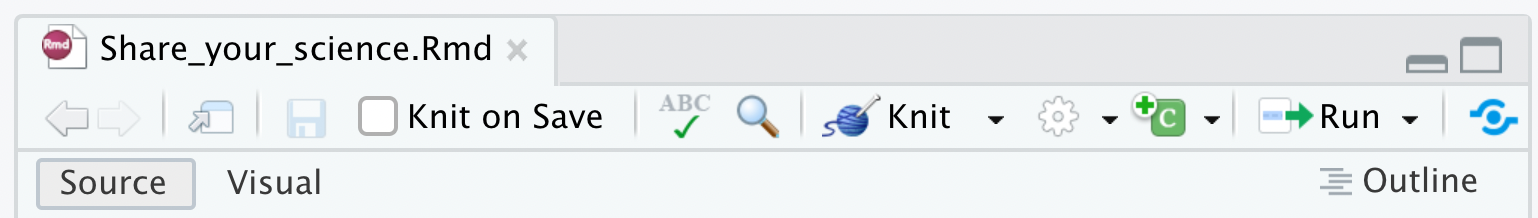
\includegraphics[width=0.5\linewidth]{figures/Knit} \end{center}

\emph{(If this did not work, perhaps you have not installed the rmarkdown or tinytex packages)}

\begin{enumerate}
\def\labelenumi{\arabic{enumi}.}
\setcounter{enumi}{2}
\tightlist
\item
  Beside the \texttt{Knit} button is an arrow. You have the option to knit to \texttt{.pdf}, \texttt{.html}, or \texttt{.docx} output. Try producing other outputs.
\end{enumerate}

\emph{(For me, producing a .docx opened Skype (clearly a bug). This was fixed by using Finder (on my Mac) to find the .docx file that I made, and selecting Open With \textgreater{} Microsoft Word)}

\begin{enumerate}
\def\labelenumi{\arabic{enumi}.}
\setcounter{enumi}{3}
\tightlist
\item
  Below are some things to try, that will help you to complete PART I. Type the code, then \texttt{Knit} to see what happens.
\end{enumerate}

\begin{itemize}
\item
  Include variables in-text by enclosing in \texttt{\$x\$}, i.e.~this renders as \(x\), which is italicized to indicate in your writing that \(x\) is a variable rather than a letter.
\item
  \href{https://ahurford.github.io/quant-guide-all-courses/data-entry.html\#loading-or-importing-data}{Load data} using R commands. \emph{(If you want to do this quickly copy and paste the command at the end of this section)}
\item
  \href{https://bookdown.org/yihui/rmarkdown/r-code.html}{Hide the code} that loads the data in the output. i.e., read about the options for r code chunks: \texttt{echo}, \texttt{include}, \texttt{message}, \texttt{warning}, \texttt{eval}, and \texttt{results}. Print the data in your output. Show both the code and the output. Try it all!
\item
  Show only your code print out. Can you do this?
\end{itemize}

\begin{verbatim}
##   Psoil Pcorn
## 1     1    64
## 2     4    71
## 3     5    54
## 4     9    81
## 5    13    93
## 6    11    76
\end{verbatim}

\begin{itemize}
\item
  Include code in-text as \texttt{\textasciigrave{}r\ x\ \textasciigrave{}}. This renders as 80 because in a hidden coding block I loaded data and assigned \texttt{x\textless{}-mean(data\$Pcorn)}. Therefore, the reported value of \(x\) = 80 is the mean phosphorous in the soil for the data I loaded in the background. If the data change, the mean reported in this document will automatically change too.
\item
  Make \href{https://bookdown.org/yihui/rmarkdown/markdown-syntax.html\#block-level-elements}{headings, subheadings}, \href{https://bookdown.org/yihui/rmarkdown/markdown-syntax.html\#inline-formatting}{bold font}, etc.
\item
  Make a \href{https://bookdown.org/yihui/rmarkdown/markdown-syntax.html\#inline-formatting}{hyperlink}.
\item
  Use latex commands to include in-text equations, i.e., \texttt{\$y\ =\ \textbackslash{}beta\_0\ +\ \textbackslash{}beta\_1\ x\$} renders as \(y = \beta_0 + \beta_1 x\); \texttt{\$\textbackslash{}frac\{dy\}\{dt\}\ =\ e\^{}x\$} renders as \(\frac{dy}{dt} = e^x\). \emph{(You may need to type \texttt{require(tinytex)} in the Console to get this to work. `The website \href{https://detexify.kirelabs.org/classify.html}{Detexify} is fun for identifying latex commands for different symbols (Some advanced symbols may require packages that you haven't installed and therfore won't work))}.
\item
  Try some \href{https://bookdown.org/yihui/rmarkdown/markdown-syntax.html\#math-expressions}{more complicated} Latex.
\end{itemize}

\begin{Shaded}
\begin{Highlighting}[]
\NormalTok{data }\OtherTok{\textless{}{-}} \FunctionTok{read.csv}\NormalTok{(}\StringTok{\textquotesingle{}https://raw.githubusercontent.com/ahurford/biol{-}4605{-}data/main/data/corn.csv\textquotesingle{}}\NormalTok{, }\AttributeTok{fill=}\ConstantTok{TRUE}\NormalTok{)}
\end{Highlighting}
\end{Shaded}

\begin{itemize}
\item
  If you would like a more structured introduction to R Markdown you can read \href{https://bookdown.org/yihui/rmarkdown/}{R Markdown: the definitive guide}.
\item
  This \href{https://www.rstudio.com/wp-content/uploads/2015/02/rmarkdown-cheatsheet.pdf}{R markdown cheat sheet} is helpful.
\item
  Some more advanced skills you might learn are making alert boxes, or changing some of the options in the \href{https://bookdown.org/yihui/rmarkdown/html-document.html}{YAML}. The alert boxes in this document are made as \texttt{div\ class="alert\ alert-info"} between \texttt{\textless{}\ \textgreater{}}, then the text, and closed with \texttt{/div} between \texttt{\textless{}\ \textgreater{}}.
\item
  My experience making tables in \texttt{.Rmd} has not been good. Usually, I make the table in \texttt{.docx}, print to \texttt{.pdf}, take a screenshot and import the \texttt{.png} to \texttt{.Rmd} or \texttt{.tex}.
\end{itemize}

\begin{enumerate}
\def\labelenumi{\arabic{enumi}.}
\setcounter{enumi}{4}
\tightlist
\item
  For your PART I specifically, you need to make a figure in \texttt{ggplot}. For \texttt{ggplot} you need your data as a data frame. The code that I used in the example was:
\end{enumerate}

\begin{Shaded}
\begin{Highlighting}[]
\NormalTok{age }\OtherTok{=} \FunctionTok{seq}\NormalTok{(}\DecValTok{1}\NormalTok{,}\DecValTok{25}\NormalTok{)}
\NormalTok{difference }\OtherTok{=} \FunctionTok{c}\NormalTok{(}\SpecialCharTok{{-}}\DecValTok{20}\NormalTok{, }\SpecialCharTok{{-}}\DecValTok{26}\NormalTok{, }\SpecialCharTok{{-}}\DecValTok{24}\NormalTok{, }\SpecialCharTok{{-}}\DecValTok{20}\NormalTok{, }\SpecialCharTok{{-}}\DecValTok{22}\NormalTok{, }\SpecialCharTok{{-}}\DecValTok{20}\NormalTok{, }\SpecialCharTok{{-}}\DecValTok{10}\NormalTok{, }\DecValTok{0}\NormalTok{,}
               \DecValTok{20}\NormalTok{, }\DecValTok{23}\NormalTok{, }\DecValTok{9}\NormalTok{, }\DecValTok{5}\NormalTok{, }\DecValTok{12}\NormalTok{, }\DecValTok{14}\NormalTok{, }\DecValTok{16}\NormalTok{, }\DecValTok{10}\NormalTok{, }\DecValTok{8}\NormalTok{, }\DecValTok{6}\NormalTok{, }\DecValTok{7}\NormalTok{, }\DecValTok{11}\NormalTok{, }\DecValTok{5}\NormalTok{, }\DecValTok{6}\NormalTok{, }\DecValTok{4}\NormalTok{, }\DecValTok{5}\NormalTok{, }\DecValTok{10}\NormalTok{)}
\NormalTok{data }\OtherTok{=} \FunctionTok{data.frame}\NormalTok{(}\AttributeTok{age=}\NormalTok{age, }\AttributeTok{difference =}\NormalTok{ difference)}
\end{Highlighting}
\end{Shaded}

As you can see, I have guessed the values in the plot and entered them manually. This is okay for the purposes of completing your assignment. (Extra for experts - try a package like \href{https://github.com/adamkucharski/scrapR}{\texttt{scrapR}} or \href{https://github.com/tpoisot/digitize}{\texttt{digitize}}).

\begin{enumerate}
\def\labelenumi{\arabic{enumi}.}
\setcounter{enumi}{5}
\tightlist
\item
  You need to install \texttt{ggplot2}. You also need to load that package because we are going to use functions from it now (do this as \texttt{require(ggplot2)}). The code that I used to make my \texttt{ggplot} was:
\end{enumerate}

\begin{Shaded}
\begin{Highlighting}[]
\NormalTok{g1}\OtherTok{=}\FunctionTok{ggplot}\NormalTok{(}\AttributeTok{data =}\NormalTok{ data, }\FunctionTok{aes}\NormalTok{(}\AttributeTok{x =}\NormalTok{ age, }\AttributeTok{y =}\NormalTok{ difference)) }\SpecialCharTok{+} 
  \FunctionTok{geom\_point}\NormalTok{() }\SpecialCharTok{+}
  \FunctionTok{geom\_line}\NormalTok{() }\SpecialCharTok{+}
  \FunctionTok{xlab}\NormalTok{(}\StringTok{"Adult Age, Days"}\NormalTok{)}\SpecialCharTok{+}
  \FunctionTok{ylab}\NormalTok{(}\StringTok{"Difference"}\NormalTok{)}
\NormalTok{g1}
\end{Highlighting}
\end{Shaded}

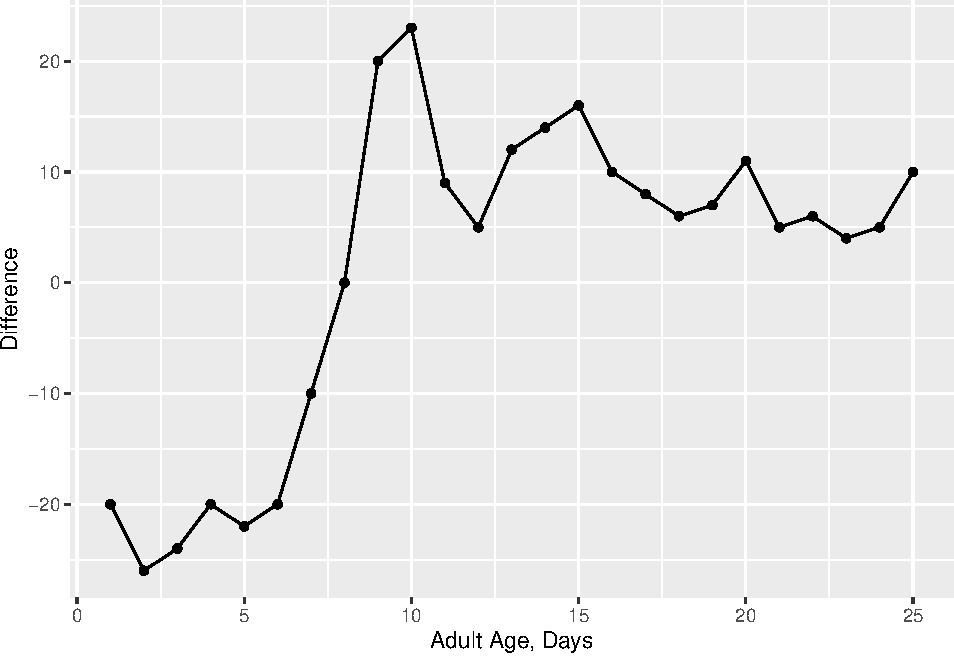
\includegraphics{BIOL-3295_files/figure-latex/unnamed-chunk-8-1.pdf}

If you need to add a title, you can add a layer \texttt{+\ ggtitle("Your\ title)}, to control the axis limits, use \texttt{+\ xlim(c(-10,10))} (with the values you need). Generally, you should be able to use an internet search to find what you need. You can also read more about \texttt{ggplot} \href{https://ahurford.github.io/quant-guide-all-courses/ggplot.html}{here}.

\begin{enumerate}
\def\labelenumi{\arabic{enumi}.}
\setcounter{enumi}{6}
\item
  To make your figure caption, just type below where your figure prints. To get bold text, use ** bold text ** (but without space between the ** and the text).
\item
  The last thing we need is to take a screenshot of the figure you are trying to reproduce, and to include it as a figure. I like to put all my figures in a folder named figure. You can read about including a \href{https://bookdown.org/yihui/rmarkdown/r-code.html\#figures}{figure} that is a \texttt{.png} or other format. Of the options, I find using knitr::include\_graphics() within a code chunk best because it seems easier to control the figure size. The code that I used in my example of how I completed PART I was:
\end{enumerate}

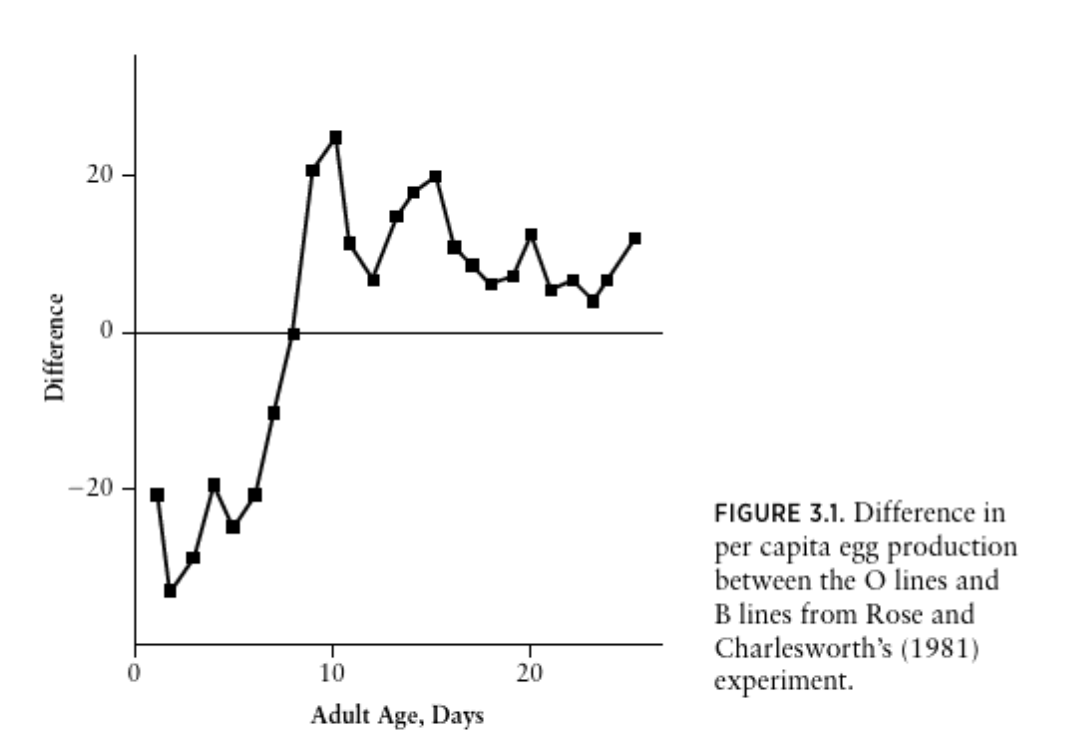
\includegraphics[width=0.9\linewidth]{figures/actual-fig}

Now you have all the information you need to complete PART I, you just need to put the pieces together. If you are stuck, ask me or a classmate.

\hypertarget{partII}{%
\chapter*{PART II - Instructions}\label{partII}}

\begin{itemize}
\item
  \href{https://ahurford.github.io/quant-guide-all-courses/install.html}{Install} the \texttt{dplyr} package, all dependencies, and load the package.
\item
  For instructions to clean data using tidyverse see \href{https://ahurford.github.io/quant-guide-all-courses/handling-data.html\#dplyr}{here}
\end{itemize}

First you need to \href{https://ahurford.github.io/quant-guide-all-courses/data-entry.html\#loading-or-importing-data}{load} the messy data from \href{https://datacarpentry.org/semester-biology/exercises/Tidy-data-improving-messy-data-SQL/}{here}.

It may be helpful to view the data in Excel to understand what it looks like before you import it to \texttt{R}.

Use \texttt{head(data)} in the Console, or \texttt{data} to view your data (where \texttt{data} is the name I gave my data).

\begin{Shaded}
\begin{Highlighting}[]
\FunctionTok{head}\NormalTok{(data)}
\end{Highlighting}
\end{Shaded}

\begin{verbatim}
##                 X          X.1       X.2      X.3    X.4 X.5            X.6
## 1                                                         NA               
## 2 Data for Site 7                                         NA               
## 3                                                         NA               
## 4         Plot: 1                                         NA        Plot: 2
## 5  Date collected       Family     Genus  Species Weight  NA Date collected
## 6        01/09/14 Heteromyidae Dipodomys merriami     40  NA       01/08/14
##          X.7     X.8      X.9   X.10 X.11           X.12             X.13
## 1                                      NA                                
## 2                                      NA                                
## 3                                      NA                                
## 4                                      NA        Plot: 3                 
## 5     Family   Genus  Species Weight   NA Date collected          Species
## 6 Cricetidae Neotoma albigula   -999   NA            1/8 Dipodomys ordii*
##     X.14
## 1       
## 2       
## 3       
## 4       
## 5 Weight
## 6     42
\end{verbatim}

These data are very messy indeed! A helpful command is to know the column names:

\begin{Shaded}
\begin{Highlighting}[]
\FunctionTok{colnames}\NormalTok{(data)}
\end{Highlighting}
\end{Shaded}

\begin{verbatim}
##  [1] "X"    "X.1"  "X.2"  "X.3"  "X.4"  "X.5"  "X.6"  "X.7"  "X.8"  "X.9" 
## [11] "X.10" "X.11" "X.12" "X.13" "X.14"
\end{verbatim}

\begin{Shaded}
\begin{Highlighting}[]
\CommentTok{\# Extract a row using tidyverse commands}
\NormalTok{dataX }\OtherTok{=}\FunctionTok{select}\NormalTok{(data, }\StringTok{"X"}\NormalTok{)}
\CommentTok{\# This is base R syntax to extract specifically rows 6 to 14}
\NormalTok{date.collected }\OtherTok{=}\NormalTok{ dataX}\SpecialCharTok{$}\NormalTok{X[}\DecValTok{6}\SpecialCharTok{:}\DecValTok{14}\NormalTok{]}
\CommentTok{\# as.Date() is needed for R to treat this variable as a date}
\NormalTok{date.collected }\OtherTok{=} \FunctionTok{as.Date}\NormalTok{(date.collected, }\AttributeTok{format =} \StringTok{"\%m/\%d/\%y"}\NormalTok{)}
\CommentTok{\# This prints to the output, so you can see what I have done}
\NormalTok{date.collected}
\end{Highlighting}
\end{Shaded}

\begin{verbatim}
## [1] "2014-01-09" "2014-01-09" "2014-01-09" "2014-01-09" "2014-01-20"
## [6] "2014-01-20" "2014-03-13" "2014-03-13" "2014-03-13"
\end{verbatim}

I will aim to make a data frame with ``date collected'' and ``weight'' for Plot 1. Inspecting the data, weight is \texttt{"X.4"} for Plot 1.

\begin{Shaded}
\begin{Highlighting}[]
\NormalTok{weight }\OtherTok{=} \FunctionTok{select}\NormalTok{(data, }\StringTok{"X.4"}\NormalTok{)}
\CommentTok{\# as.numeric() is needed because otherwise R doesn\textquotesingle{}t recognize these data as numbers {-} which I need for the multiplication later}
\NormalTok{weight }\OtherTok{=} \FunctionTok{as.numeric}\NormalTok{(weight}\SpecialCharTok{$}\NormalTok{X}\FloatTok{.4}\NormalTok{[}\DecValTok{6}\SpecialCharTok{:}\DecValTok{14}\NormalTok{])}
\CommentTok{\# Make this into a data frame so I can plot using ggplot}
\NormalTok{cleaned.data }\OtherTok{=} \FunctionTok{data.frame}\NormalTok{(date.collected, weight)}
\CommentTok{\# add a column that is a mutated column}
\NormalTok{cleaned.data }\OtherTok{=} \FunctionTok{mutate}\NormalTok{(cleaned.data,}\AttributeTok{weight.kg =}\NormalTok{ weight}\SpecialCharTok{/}\DecValTok{1000}\NormalTok{)}
\CommentTok{\# print the cleaned data so we can see what it looks like}
\NormalTok{cleaned.data}
\end{Highlighting}
\end{Shaded}

\begin{verbatim}
##   date.collected weight weight.kg
## 1     2014-01-09     40     0.040
## 2     2014-01-09     36     0.036
## 3     2014-01-09    135     0.135
## 4     2014-01-09     39     0.039
## 5     2014-01-20     43     0.043
## 6     2014-01-20    144     0.144
## 7     2014-03-13     51     0.051
## 8     2014-03-13     44     0.044
## 9     2014-03-13    146     0.146
\end{verbatim}

Now the data is in a format that I can make a plot:

\begin{Shaded}
\begin{Highlighting}[]
\FunctionTok{require}\NormalTok{(ggplot2)}
\NormalTok{g1}\OtherTok{=}\FunctionTok{ggplot}\NormalTok{(}\AttributeTok{data =}\NormalTok{ cleaned.data, }\FunctionTok{aes}\NormalTok{(}\AttributeTok{x =}\NormalTok{ date.collected, }\AttributeTok{y =}\NormalTok{ weight.kg)) }\SpecialCharTok{+} 
  \FunctionTok{geom\_point}\NormalTok{() }\SpecialCharTok{+}
  \FunctionTok{geom\_line}\NormalTok{() }\SpecialCharTok{+}
  \FunctionTok{xlab}\NormalTok{(}\StringTok{"Date collected"}\NormalTok{)}\SpecialCharTok{+}
  \FunctionTok{ylab}\NormalTok{(}\StringTok{"Weight in kg"}\NormalTok{)}
\NormalTok{g1}
\end{Highlighting}
\end{Shaded}

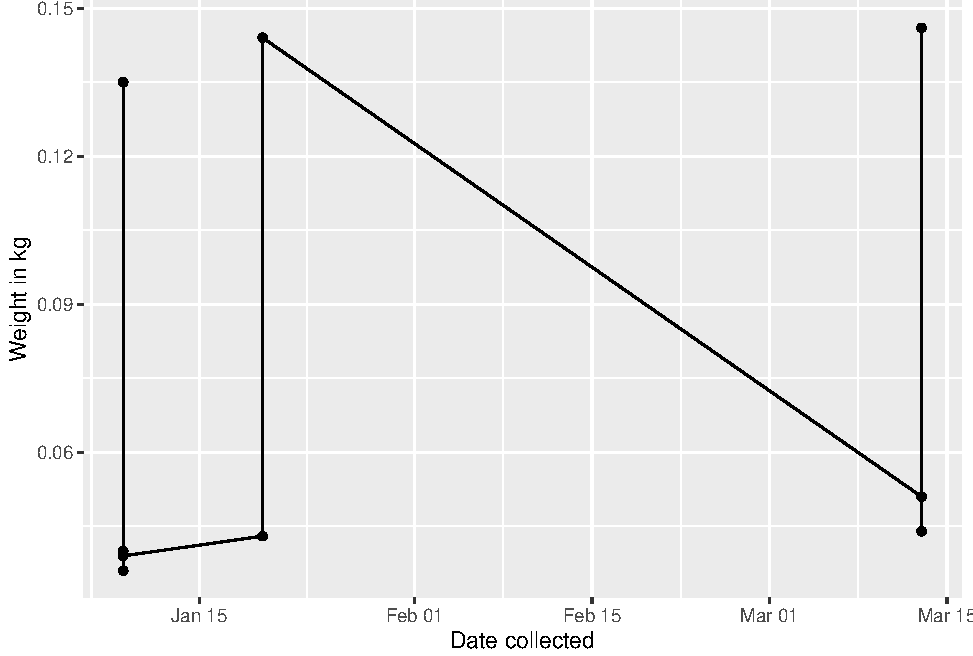
\includegraphics{BIOL-3295_files/figure-latex/unnamed-chunk-14-1.pdf}

\end{document}
